\documentclass[UTF8]{article}
\usepackage{graphicx}
\usepackage{subfigure}
\usepackage{amsmath}
\usepackage{makecell}
\usepackage[utf8]{inputenc}
\usepackage[space]{ctex} %中文包
\usepackage{listings} %放代码
\usepackage{xcolor} %代码着色宏包
\usepackage{CJK} %显示中文宏包
\usepackage{float}
\usepackage{diagbox}
\usepackage{bm}
\usepackage{ulem} 
\usepackage{amssymb}
\usepackage{soul}
\usepackage{color}
\usepackage{geometry}
\usepackage{fancybox} %花里胡哨的盒子
\usepackage{xhfill} %填充包, 可画分割线 https://www.latexstudio.net/archives/8245
\usepackage{multicol} %多栏包
\usepackage{enumerate} %可以方便地自定义枚举标题
\usepackage{multirow} %表格中多行单元格合并
\usepackage{wasysym} %可以使用wasysym里的一堆奇奇怪怪的符号
\usepackage{hyperref} % url
%%%%%%%%%%%%%%%伪代码%%%%%%%%%%%%%%%
\usepackage{amsmath}
\usepackage{algorithm}
\usepackage[noend]{algpseudocode}
%%%%%%%%%%%%%%%画图包%%%%%%%%%%%%%%%
\usepackage{tikz}
\usepackage{pgfplots} % http://pgfplots.sourceforge.net/gallery.html
\usetikzlibrary{pgfplots.patchplots} % 拟合支持
\usetikzlibrary{arrows,shapes,automata,petri,positioning,calc} % 状态图支持
\usetikzlibrary{arrows.meta} % 箭头
\usetikzlibrary{shadows} % 阴影支持
\usepackage{forest} % 画树

\geometry{left = 1.5cm, right = 1.5cm, top=1.5cm, bottom=2cm}

\definecolor{mygreen}{rgb}{0,0.6,0}
\definecolor{mygray}{rgb}{0.5,0.5,0.5}
\definecolor{mymauve}{rgb}{0.58,0,0.82}
\lstset{
	backgroundcolor=\color{white}, 
	%\tiny < \scriptsize < \footnotesize < \small < \normalsize < \large < \Large < \LARGE < \huge < \Huge
	basicstyle = \footnotesize,       
	breakatwhitespace = false,        
	breaklines = true,                 
	captionpos = b,                    
	commentstyle = \color{mygreen}\bfseries,
	extendedchars = false,
	frame = shadowbox, 
	framerule=0.5pt,
	keepspaces=true,
	keywordstyle=\color{blue}\bfseries, % keyword style
	language = C++,                     % the language of code
	otherkeywords={string}, 
	numbers=left, 
	numbersep=5pt,
	numberstyle=\tiny\color{mygray},
	rulecolor=\color{black},         
	showspaces=false,  
	showstringspaces=false, 
	showtabs=false,    
	stepnumber=1,         
	stringstyle=\color{mymauve},        % string literal style
	tabsize=4,          
	title=\lstname           
}

%\sum\nolimits_{j=1}^{M}   上下标位于求和符号的水平右端,
%\sum\limits_{j=1}^{M}   上下标位于求和符号的上下处,
%\sum_{j=1}^{M}  对上下标位置没有设定,会随公式所处环境自动调整。

%%%%%%%%%%%%%画图包%%%%%%%%%%%%%
\usepackage{tikz}
%%%%%%%%%%%%%好看的矩形%%%%%%%%%%%%%
\tikzset{
  rect1/.style = {
    shape = rectangle,% 指定样式
    minimum height=2cm,% 最小高度
    minimum width=4cm,% 最小宽度
    align = center,% 文字居中
    drop shadow,% 阴影
  }
}
%%%%%%%%%%%%%画图背景包%%%%%%%%%%%%%
\usetikzlibrary{backgrounds}

%%%%%%%%%%%%%在tikz中画一个顶点%%%%%%%%%%%%%
%%%%%%%%%%%%%#1:node名称%%%%%%%%%%%%%
%%%%%%%%%%%%%#2:位置%%%%%%%%%%%%%
%%%%%%%%%%%%%#3:标签%%%%%%%%%%%%%
\newcommand{\newVertex}[3]{\node[circle, draw=black, line width=1pt, scale=0.8] (#1) at #2{#3}}
%%%%%%%%%%%%%在tikz中画一条边%%%%%%%%%%%%%
\newcommand{\newEdge}[2]{\draw [black,very thick](#1)--(#2)}
%%%%%%%%%%%%%在tikz中放一个标签%%%%%%%%%%%%%
%%%%%%%%%%%%%#1:名称%%%%%%%%%%%%%
%%%%%%%%%%%%%#2:位置%%%%%%%%%%%%%
%%%%%%%%%%%%%#3:标签内容%%%%%%%%%%%%%
\newcommand{\newLabel}[3]{\node[line width=1pt] (#1) at #2{#3}}

%%%%%%%%%%%%%强制跳过一行%%%%%%%%%%%%%
\newcommand{\jumpLine} {\hspace*{\fill} \par}
%%%%%%%%%%%%%关键点指令,可用itemise替代%%%%%%%%%%%%%
\newcommand{\average}[1]{\left\langle #1\right\rangle }
%%%%%%%%%%%%%表格内嵌套表格%%%%%%%%%%%%%
\newcommand{\keypoint}[2]{$\bullet$\textbf{#1}\quad#2\par}
%%%%%%%%%%%%%<T>平均值表示%%%%%%%%%%%%%
\newcommand{\tabincell}[2]{\begin{tabular}{@{}#1@{}}#2\end{tabular}}%放在导言区
%%%%%%%%%%%%%大黑点item头%%%%%%%%%%%%%
\newcommand{\itemblt}{\item[$\bullet$]}
%%%%%%%%%%%%%大圈item头%%%%%%%%%%%%%
\newcommand{\itemc}{\item[$\circ$]}
%%%%%%%%%%%%%大星星item头%%%%%%%%%%%%%
\newcommand{\itembs}{\item[$\bigstar$]}
%%%%%%%%%%%%%右▷item头%%%%%%%%%%%%%
\newcommand{\itemrhd}{\item[$\rhd$]}
%%%%%%%%%%%%%定义为%%%%%%%%%%%%%
\newcommand{\defas}{=_{df}}
%%%%%%%%%%%%%偏导%%%%%%%%%%%%%
\newcommand{\partialx}[2]{\frac{\partial #1}{\partial #2}}
%%%%%%%%%%%%%蕴含%%%%%%%%%%%%%
\newcommand{\imp}{\rightarrow}
%%%%%%%%%%%%%上取整%%%%%%%%%%%%%
\newcommand{\ceil}[1]{\lceil#1\rceil}
%%%%%%%%%%%%%下取整%%%%%%%%%%%%%
\newcommand{\floor}[1]{\lfloor#1\rfloor}
%%%%%%%%%%%%%textbullet%%%%%%%%%%%%%
\newcommand{\blt}{\bullet}
%%%%%%%%%%%%%右箭头上加字%%%%%%%%%%%%%
\newcommand{\righttextarrow}[1]{\stackrel{#1}{\longrightarrow}}
%%%%%%%%%%%%%左箭头上加字%%%%%%%%%%%%%
\newcommand{\lefttextarrow}[1]{\stackrel{#1}{\longleftarrow}}

%%%%%%%%%%%%%双线分割线%%%%%%%%%%%%%
\newcommand*{\doublerule}{\hrule width \hsize height 1pt \kern 0.5mm \hrule width \hsize height 2pt}
%%%%%%%%%%%%%双线中间可加东西的分割线%%%%%%%%%%%%%
\newcommand\doublerulefill{\leavevmode\leaders\vbox{\hrule width .1pt\kern1pt\hrule}\hfill\kern0pt }
%%%%%%%%%%%%%左大括号%%%%%%%%%%%%%
\newcommand{\leftbig}[1]{\left\{\begin{array}{l}#1\end{array}\right.}
%%%%%%%%%%%%%矩阵%%%%%%%%%%%%%
\newcommand{\mat}[2]{\left[\begin{array}{#1}#2\end{array}\right]}
%%%%%%%%%%%%%可换行圆角文本框%%%%%%%%%%%%%
\newcommand{\ovalboxn}[1]{\ovalbox{\tabincell{l}{#1}}}
%%%%%%%%%%%%%设置section的counter, 使从1开始%%%%%%%%%%%%%
\setcounter{section}{0}

%%%%%%%%%%%%%Colors%%%%%%%%%%%%%
\newcommand{\lightercolor}[3]{% Reference Color, Percentage, New Color Name
    \colorlet{#3}{#1!#2!white}
}
\newcommand{\darkercolor}[3]{% Reference Color, Percentage, New Color Name
    \colorlet{#3}{#1!#2!black}
}
\definecolor{aquamarine}{rgb}{0.5, 1.0, 0.83}
\definecolor{Seashell}{RGB}{255, 245, 238} %背景色浅一点的
\definecolor{Firebrick4}{RGB}{255, 0, 0}%文字颜色红一点的
\lightercolor{gray}{20}{lgray}
\newcommand{\hlg}[1]{
	\begingroup
		\sethlcolor{lgray}%背景色
		\textcolor{black}{\hl{\mbox{#1}}}%textcolor里面对应文字颜色
	\endgroup
}



\title{编译原理与技术 H4-2}
\date{}
\author{PB18111697 王章瀚}

\begin{document}
\maketitle
\section*{1}
\noindent LR分析与LALR分析的比较
\subsection*{1)}
\noindent 请分别给出终结符串 bbabba 以及 bba 的LR分析过程, 说明规范的LR分析不会把错误的符号移进栈.
\begin{figure}[H]
	\centering
	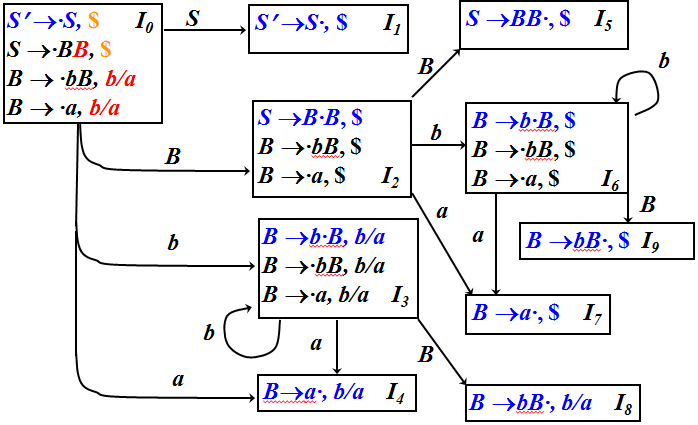
\includegraphics[width=\linewidth/2]{1a.png}
\end{figure}\par
\subsubsection*{对于bbabba}
\noindent 过程列表如下:\\
\begin{center}
\begin{tabular}{|c|c|c|c|c|}
\hline
 & 栈 & 符号 & 输入 & 动作 \\
\hline
1 & 0 &  & $bbabba\$$ & 移进 \\
\hline
2 & 0 3 & $b$ & $babba\$$ & 移进 \\
\hline
3 & 0 3 3 & $bb$ & $abba\$$ & 移进 \\
\hline
4 & 0 3 3 4 & $bba$ & $bba\$$ & 按$B\rightarrow a$归约 \\
\hline
5 & 0 3 3 8 & $bbB$ & $bba\$$ & 按$B\rightarrow bB$归约 \\
\hline
6 & 0 3 8 & $bB$ & $bba\$$ & 按$B\rightarrow bB$归约 \\
\hline
7 & 0 2 & $B$ & $bba\$$ & 移进 \\
\hline
8 & 0 2 6 & $Bb$ & $ba\$$ & 移进 \\
\hline
9 & 0 2 6 6 & $Bbb$ & $a\$$ & 移进 \\
\hline
10 & 0 2 6 6 7 & $Bbba$ & $\$$ & 按$B\rightarrow a$归约 \\
\hline
11 & 0 2 6 6 9 & $BbbB$ & $\$$ & 按$B\rightarrow a$归约 \\
\hline
12 & 0 2 6 9 & $BbB$ & $\$$ & 按$B\rightarrow bB$归约 \\
\hline
13 & 0 2 5 & $BB$ & $\$$ & 按$S\rightarrow BB$归约 \\
\hline
14 & 0 1 & $S$ & $\$$ & 接受 \\
\hline
\end{tabular}
\end{center}

\subsubsection*{对于bba}
\noindent 过程列表如下:\\
\begin{center}
\begin{tabular}{|c|c|c|c|c|}
\hline
 & 栈 & 符号 & 输入 & 动作 \\
\hline
1 & 0 &  & $bbabba\$$ & 移进 \\
\hline
2 & 0 3 & $b$ & $ba\$$ & 移进 \\
\hline
3 & 0 3 3 & $bb$ & $a\$$ & 移进 \\
\hline
4 & 0 3 3 4 & $bba$ & $\$$ & 报告错误 \\
\hline
\end{tabular}
\end{center}
由此可以看出来, LR(1)不会移进错误的符号. \\
原因在于
\begin{itemize}
	\item LR(1)提前看了一位, 并且LR(1)的项目搜索符是根据已有项目及{\sc First}函数确定的(这里《编译原理 第3版》\footnote{《编译原理》第3版, 陈意云, 张昱编著}上第82页有所描述), 如果确认不是正确的搜索符, 就会立马发现有问题而报错. 因此它必然不会移入错误的符号.例如此题中, 在$I_4$状态下, 需要满足下一位是$b/a$才去进行归约, 但下一位是$\$$, 因此直接报错, 并不会移进$\$$.
	\item 此外, 虽然LALR也提前看了一位, 但它是经过合并的, 也就是说会出现比如:原本状态1和状态2合并成状态12, 而状态1经过符号x有某action, 状态2没有, 那么合并之后, 即使是状态2, 也会认为可以经过x有这个action, 因此不能及时排除错误. 也就是说LALR经过合并, 其信息更少了.
\end{itemize}

\subsection*{2)}
\noindent 请给出终结符串 bbabba 的LALR分析过程,并结合分析过程指出LALR分析相比LR分析的差异
\begin{figure}[H]
	\centering
	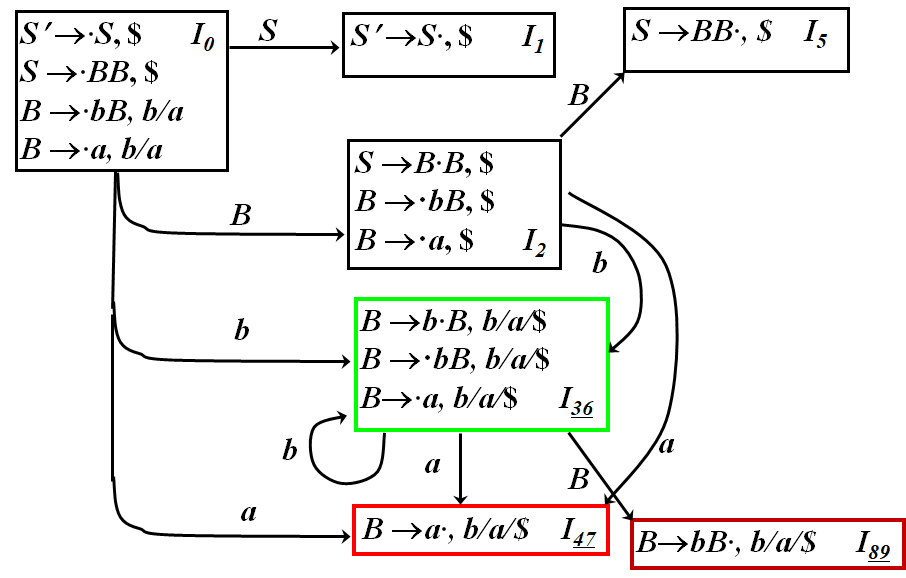
\includegraphics[width=\linewidth/2]{1b.png}
\end{figure}\par
\noindent 过程列表如下:\\
\begin{center}
\begin{tabular}{|c|c|c|c|c|}
\hline
 & 栈 & 符号 & 输入 & 动作 \\
\hline
1 & 0 &  & $bbabba\$$ & 移进 \\
\hline
2 & 0 36 & $b$ & $babba\$$ & 移进 \\
\hline
3 & 0 36 36 & $bb$ & $abba\$$ & 移进 \\
\hline
4 & 0 36 36 47 & $bba$ & $bba\$$ & 按$B\rightarrow a$归约 \\
\hline
5 & 0 36 36 89 & $bbB$ & $bba\$$ & 按$B\rightarrow bB$归约 \\
\hline
6 & 0 36 89 & $bB$ & $bba\$$ & 按$B\rightarrow bB$归约 \\
\hline
7 & 0 2 & $B$ & $bba\$$ & 移进 \\
\hline
8 & 0 2 36 & $Bb$ & $ba\$$ & 移进 \\
\hline
9 & 0 2 36 36 & $Bbb$ & $a\$$ & 移进 \\
\hline
10 & 0 2 36 36 47 & $Bbba$ & $\$$ & 按$B\rightarrow a$归约 \\
\hline
11 & 0 2 36 36 89 & $BbbB$ & $\$$ & 按$B\rightarrow a$归约 \\
\hline
12 & 0 2 36 89 & $BbB$ & $\$$ & 按$B\rightarrow bB$归约 \\
\hline
13 & 0 2 5 & $BB$ & $\$$ & 按$S\rightarrow BB$归约 \\
\hline
14 & 0 1 & $S$ & $\$$ & 接受 \\
\hline
\end{tabular}
\end{center}
\textbf{差异分析}: 由此可见, 分析过程除了状态的编号有差异(变为合并了的编号), 其他地方并没有区别. 但这能够很好地节省空间与状态数, 有利于优化分析器性能.

\newpage
\section*{2}
\noindent 教材3.31: 下面两个文法中哪一个不是LR(1)文法? 对非LR(1)的那个文法, 给出那个有移进-归约冲突的规范的LR(1)项目集.\\
\begin{minipage}{\linewidth/3}
$$\begin{array}{l}
S\rightarrow aAc\\
A\rightarrow Abb|b
\end{array}$$
\end{minipage}
\begin{minipage}{\linewidth/3}
$$\begin{array}{l}
S\rightarrow aAc\\
A\rightarrow bAb|b
\end{array}$$
\end{minipage}
\subsection*{先给出结论}
\noindent 右边的(即第二个)文法不是LR(1)文法, 有移进-规约冲突, 这个项目集为如下:
	$$I_7\left\{\begin{array}{ll}
	A\rightarrow b\blt Ab & ,b\\
	A\rightarrow b\blt & ,b\\
	A\rightarrow \blt bAb & ,b\\
	A\rightarrow \blt b & ,b\\
	\end{array}\right.$$
\subsection*{(1). 考虑第一个文法}
\begin{itemize}
\item 拓广文法
	$$\begin{array}{ll}
	  & S'\rightarrow S\\
	1 & S\rightarrow aAc\\
	2 & A\rightarrow Abb\\
	3 & A\rightarrow b
	\end{array}$$
\item LR(1)项目集规范族
	\begin{itemize}
	\item 首先是$I_0$
		$$I_0\left\{\begin{array}{ll}
		S'\rightarrow \blt S & ,\$ \\
		S\rightarrow \blt aAc & ,\$ \\
		\end{array}\right.$$
	\item 从$I_0$出发
		\begin{itemize}
		\item 考虑$goto(I_0,S)$
			$$I_1\left\{\begin{array}{ll}
			S'\rightarrow  S\blt & ,\$\\
			\end{array}\right.$$
		\item 考虑$goto(I_0,a)$
			$$I_2\left\{\begin{array}{ll}
			S\rightarrow a\blt Ac & ,\$ \\
			A\rightarrow \blt Abb & , b/c\\
			A\rightarrow \blt b & , b/c\\
			\end{array}\right.$$
		\end{itemize}
	\item 从$I_1$无了
	\item 从$I_2$出发
		\begin{itemize}
		\item 考虑$goto(I_2,A)$
			$$I_3\left\{\begin{array}{ll}
			S\rightarrow aA\blt c & ,\$ \\
			A\rightarrow A\blt bb & , b/c\\
			\end{array}\right.$$
		\item 考虑$goto(I_2,b)$
			$$I_4\left\{\begin{array}{ll}
			A\rightarrow b\blt & , b/c\\
			\end{array}\right.$$
		\end{itemize}
	\item 从$I_3$出发
		\begin{itemize}
		\item 考虑$goto(I_3,c)$
			$$I_5\left\{\begin{array}{ll}
			S\rightarrow aAc\blt & ,\$ \\
			\end{array}\right.$$
		\item 考虑$goto(I_3,b)$
			$$I_6\left\{\begin{array}{ll}
			A\rightarrow Ab\blt b & , b/c\\
			\end{array}\right.$$
		\end{itemize}
	\item 从$I_4,I_5$均无
	\item 从$I_6$, 考虑$goto(I_6,b)$
		$$I_7\left\{\begin{array}{ll}
		A\rightarrow Abb\blt & , b/c\\
		\end{array}\right.$$
	\end{itemize}
\item 尝试构造action函数
	\begin{center}
	\begin{tabular}{|c|c|c|c|c|}
	\hline
	 & a & b & c & \$ \\
	\hline
	0 & s2 &  &  &  \\
	\hline
	1 &  &  &  & acc \\
	\hline
	2 &  & s4 &  &  \\
	\hline
	3 &  & s6 & s5 &  \\
	\hline
	4 &  & r3 & r3 &  \\
	\hline
	5 &  &  &  & r1 \\
	\hline
	6 &  & s7 &  &  \\
	\hline
	7 &  & r2 & r2 &  \\
	\hline
	\end{tabular}
	\end{center}
	\hlg{\textbf{构造过程中没有造成任何冲突, 因此可以认定该文法是LR(1)的.}}
\end{itemize}

\subsection*{(2). 考虑第二个文法}

\begin{itemize}
\item 拓广文法
	$$\begin{array}{ll}
	  & S'\rightarrow S\\
	1 & S\rightarrow aAc\\
	2 & A\rightarrow bAb\\
	3 & A\rightarrow b
	\end{array}$$
\item LR(1)项目集规范族
	\begin{itemize}
	\item 首先是$I_0$
		$$I_0\left\{\begin{array}{ll}
		S'\rightarrow \blt S & ,\$ \\
		S\rightarrow \blt aAc & ,\$ \\
		\end{array}\right.$$
	\item 从$I_0$出发
		\begin{itemize}
		\item 考虑$goto(I_0,S)$
			$$I_1\left\{\begin{array}{ll}
			S'\rightarrow S\blt & ,\$ \\
			\end{array}\right.$$
		\item 考虑$goto(I_0,S)$
			$$I_2\left\{\begin{array}{ll}
			S\rightarrow a\blt Ac & ,\$ \\
			A\rightarrow \blt bAb & ,c\\
			A\rightarrow \blt b & ,c\\
			\end{array}\right.$$
		\end{itemize}
	\item 从$I_1$无了
	\item 从$I_2$出发
		\begin{itemize}
		\item 考虑$goto(I_2,A)$
			$$I_3\left\{\begin{array}{ll}
			S\rightarrow aA\blt c & ,\$ \\
			\end{array}\right.$$
		\item 考虑$goto(I_2,b)$
			$$I_4\left\{\begin{array}{ll}
			A\rightarrow b\blt Ab & ,c\\
			A\rightarrow b\blt & ,c\\
			A\rightarrow \blt bAb & ,b\\
			A\rightarrow \blt b & ,b\\
			\end{array}\right.$$
		\end{itemize}
	\item 从$I_3$, 考虑$goto(I_3,c)$
		$$I_5\left\{\begin{array}{ll}
		S\rightarrow aAc\blt & ,\$ \\
		\end{array}\right.$$
	\item 从$I_4$出发, 
		\begin{itemize}
		\item 考虑$goto(I_4,A)$
			$$I_6\left\{\begin{array}{ll}
			A\rightarrow bA\blt b & ,c\\
			\end{array}\right.$$
		\item 考虑$goto(I_4,b)$
			$$I_7\left\{\begin{array}{ll}
			A\rightarrow b\blt Ab & ,b\\
			A\rightarrow b\blt & ,b\\
			A\rightarrow \blt bAb & ,b\\
			A\rightarrow \blt b & ,b\\
			\end{array}\right.$$
		\end{itemize}
	\item 从$I_5$, 无
	\item 从$I_6$, 考虑$goto(I_6,b)$
		$$I_8\left\{\begin{array}{ll}
		A\rightarrow bAb\blt & ,c\\
		\end{array}\right.$$
	\item 从$I_7$出发
		\begin{itemize}
		\item 考虑$goto(I_7, A)$
			$$I_9\left\{\begin{array}{ll}
			A\rightarrow bA\blt b & ,b\\
			\end{array}\right.$$
		\item 考虑$goto(I_7,b)$, 得到$I_7$
		\end{itemize}
	\item 从$I_8$, 无
	\item 从$I_9$, 考虑$goto(I_9,b)$
		$$I_{10}\left\{\begin{array}{ll}
		A\rightarrow bAb\blt & ,b\\
		\end{array}\right.$$
	\end{itemize}
\item 尝试构造action函数
	\begin{tabular}{|c|c|c|c|c|}
	\hline
	 & a & b & c & \$ \\
	\hline
	0 &  &  &  &  \\
	\hline
	1 &  &  &  & acc \\
	\hline
	2 &  & s4 &  &  \\
	\hline
	3 &  &  & s5 &  \\
	\hline
	4 &  & s7 & r3 &  \\
	\hline
	5 &  &  &  & r1 \\
	\hline
	6 &  & s8 &  &  \\
	\hline
	7 &  & s7/r3 &  &  \\
	\hline
	8 &  &  & r2 &  \\
	\hline
	9 &  & s9 &  &  \\
	\hline
	10 &  & r2 &  &  \\
	\hline
	\end{tabular}
\end{itemize}
\hlg{\textbf{可见在状态7, 若考虑b, 则会有移进归约冲突}}, 冲突项目集为

$$I_7\left\{\begin{array}{ll}
A\rightarrow b\blt Ab & ,b\\
A\rightarrow b\blt & ,b\\
A\rightarrow \blt bAb & ,b\\
A\rightarrow \blt b & ,b\\
\end{array}\right.$$

\end{document}





